%!TEX root = Lefley - Mesh to voxel transformations for optimised physics-based interactions.tex
\null\cleardoublepage
\chapter{Conclusions}

A functioning pipeline for dynamic physics-based fragmentation of objects based on their computed volumetric definition has been implemented, titled Dynamic Volumetric Fragmentation. This implementation can demonstrably be used with a physics engine to resolve post-collision fragmentation in a visually accurate manner, with further physical accuracy left as a possibility.

The problem of splitting an object precisely into fragments given only rigid mesh information has been solved by finding the entire enclosed volume as a scalar field at runtime. Partitioning of this scalar field algorithmically for each point in the field allows mass to be attributed to each fragment according to predefined rules inspired by real world physical principles.

While this implementation of DVF is not viable for real-time applications, a possible plan for achieving real-time suitability has also been outlined, focussing on parallelism.

DVF could be used in the field of Computer-Generated Imagery, where frame render times are generally much higher and do not have to be viewed in real-time. This would allow objects to be accurately fragmented without the need for an artist's input.

Continuations which would further improve the viability of DVF have been discussed in Section~\ref{sect:cont}.

\medskip

\centerline{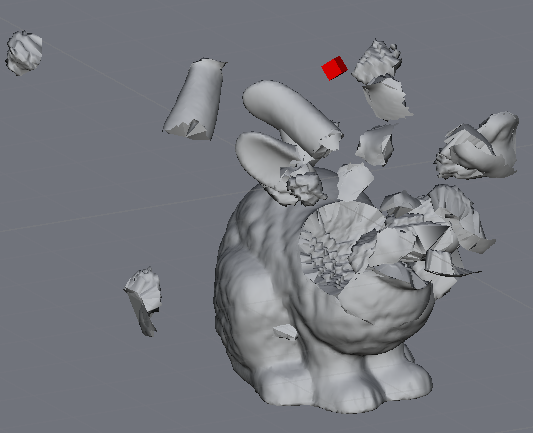
\includegraphics[scale=0.7]{voxel_exploded.png}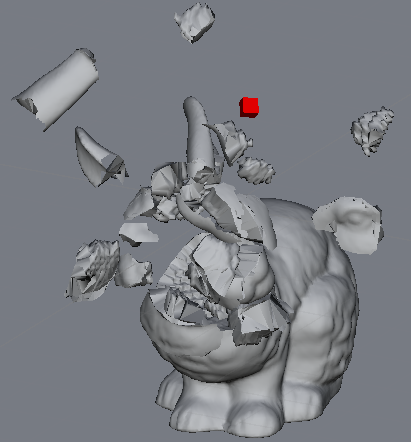
\includegraphics[scale=0.686]{voxel_exploded2.png}}